\documentclass{article}

% if you need to pass options to natbib, use, e.g.:
% \PassOptionsToPackage{numbers, compress}{natbib}
% before loading nips_2018

% ready for submission
\usepackage[final]{nips_2018}

% to compile a preprint version, e.g., for submission to arXiv, add
% add the [preprint] option:
% \usepackage[preprint]{nips_2018}

% to compile a camera-ready version, add the [final] option, e.g.:
% \usepackage[final]{nips_2018}

% to avoid loading the natbib package, add option nonatbib:
% \usepackage[nonatbib]{nips_2018}

\usepackage[utf8]{inputenc} % allow utf-8 input
\usepackage[T1]{fontenc}    % use 8-bit T1 fonts
\usepackage{hyperref}       % hyperlinks
\usepackage{url}            % simple URL typesetting
\usepackage{booktabs}       % professional-quality tables
\usepackage{amsfonts}       % blackboard math symbols
\usepackage{nicefrac}       % compact symbols for 1/2, etc.
\usepackage{microtype}      % microtypography
\usepackage{stmaryrd}

\newcommand{\theHalgorithm}{\arabic{algorithm}}
\newcommand{\sem}[1]{\llbracket{} #1 \rrbracket{}}

\newcommand{\system}{\textsc{EC$^2$} }
\newcommand{\systemEnding}{\textsc{EC$^2$}}

\newcommand{\lowerBound}{\mathscr{L}}
\newcommand{\code}[1]{{\footnotesize\texttt{#1}}}
\newcommand{\codechar}[1]{{\footnotesize{\texttt{``#1''}}}}

\usepackage{xcolor}
\definecolor{pop1}{HTML}{1F78b4}
\definecolor{pop2}{HTML}{297F23}
\definecolor{pop3}{HTML}{d95F02}
\definecolor{orange}{HTML}{d95F02}
\definecolor{teal}{HTML}{1b9e77}
\newcommand{\pop}[1]{\textcolor{pop1}{#1}}
\newcommand{\popp}[1]{\textcolor{pop2}{#1}}
\newcommand{\tree}[1]{\textcolor{pop3}{#1}}
\newcommand{\orange}[1]{\textcolor{orange}{#1}}
\newcommand{\teal}[1]{\textcolor{teal}{#1}}

\usepackage{mathrsfs}
\usepackage{listings}
\usepackage{amsthm}

\usepackage{subfig} 
\usepackage{fancyvrb}


\usepackage{caption}
\usepackage{amssymb}
\usepackage{listings}
\usepackage{wrapfig}
\usepackage{tabularx}


\usepackage{verbatim}
 \usepackage{booktabs}
 % For algorithms
\usepackage{algorithm}
\usepackage{algorithmic}
\usepackage{tikz}
\usepackage{circuitikz}
\usetikzlibrary{fit,bayesnet}
\usepackage{dsfont}
\usepackage{amsmath}
\usetikzlibrary{trees}

\DeclareMathOperator*{\argmin}{arg\,min} % thin space, limits underneath in displays
\DeclareMathOperator*{\argmax}{arg\,max} % thin space, limits underneath in displays
 


% Packages hyperref and algorithmic misbehave sometimes.  We can fix
% this with the following command.

\newcommand{\Expect}{\mathds{E}} %{{\rm I\kern-.3em E}}
\newcommand{\indicator}{\mathds{1}} %{{\rm I\kern-.3em E}}
\newcommand{\expect}{\mathds{E}} %{{\rm I\kern-.3em E}}
\newcommand{\probability}{\mathds{P}} %{{\rm I\kern-.3em P}}

\title{Library Learning in Neurally-Guided Bayesian Program Induction}

% The \author macro works with any number of authors. There are two
% commands used to separate the names and addresses of multiple
% authors: \And and \AND.
%
% Using \And between authors leaves it to LaTeX to determine where to
% break the lines. Using \AND forces a line break at that point. So,
% if LaTeX puts 3 of 4 authors names on the first line, and the last
% on the second line, try using \AND instead of \And before the third
% author name.

\author{
  Kevin Ellis\\MIT\\\texttt{ellisk@mit.edu}\And Lucas Morales\\MIT\\\texttt{lucasem@mit.edu}\And Mathias Sabl\'e-Meyer\\ENS Paris-Saclay\\\texttt{mathsm@mit.edu}
  \AND
  Armando Solar-Lezama\\MIT\\\texttt{asolar@csail.mit.edu}\And Joshua B. Tenenbaum\\MIT\\\texttt{jbt@mit.edu}
  %% \And
  %% Coauthor \\
  %% Affiliation \\
  %% Address \\
  %% \texttt{email} \\
  %% \AND
  %% Coauthor \\
  %% Affiliation \\
  %% Address \\
  %% \texttt{email} \\
  %% \And
  %% Coauthor \\
  %% Affiliation \\
  %% Address \\
  %% \texttt{email} \\
  %% \And
  %% Coauthor \\
  %% Affiliation \\
  %% Address \\
  %% \texttt{email} \\
}

\begin{document}
% \nipsfinalcopy is no longer used

\maketitle

\begin{abstract}
  Successful approaches to program induction require a hand-engineered
  domain-specific language (DSL), constraining the space of allowed
  programs and imparting prior knowledge of the domain.  We contribute
  a program induction algorithm called \system that learns a DSL while
  jointly training a neural network to efficiently search for programs
  in the learned DSL.\@ We use our model to synthesize functions on lists,
  edit text, and solve symbolic regression problems, showing how the
  model learns a domain-specific library of program components for
  expressing solutions to problems in the domain.
\end{abstract}


\section{Introduction}

Much of everyday human thinking and learning can be understood in
terms of program induction: constructing a procedure that maps inputs
to desired outputs, based on observing example input-output pairs.
People can induce programs flexibly across many different domains, and
remarkably, often from just one or a few examples.  For instance, if
shown that a text-editing program should map ``Jane Morris Goodall''
to ``J. M. Goodall'', we can guess it maps ``Richard Erskine Leakey''
to ``R. E. Leakey''; if instead the first input mapped to
``Dr. Jane'', ``Goodall, Jane'', or ''Morris'', we might have guessed
the latter should map to ``Dr. Richard'', ``Leakey, Richard'', or
``Erskine'', respectively.

The FlashFill system~\cite{gulwani2011automating} developed by
Microsoft researchers and now embedded in Excel solves problems such
as these and is probably the best known practical program-induction
algorithm, but researchers in programming languages and AI have built
successful program induction algorithms for many applications, such as
handwriting recognition and generation~\cite{lake2015human},
procedural graphics~\cite{ellis2017learning}, cognitive
modeling~\cite{DBLP:journals/cogsr/SchmidK11}, question
answering~\cite{johnson2017clevr} and robot motion
planning~\cite{devlin2017neural}, to name just a few.  These systems
work in different ways, but most hinge upon having a carefully
engineered \textbf{Domain Specific Language (DSL)}.  This is
especially true for systems such as FlashFill that aim to induce a
wide range of programs very quickly, in a few seconds or less.  DSLs
constrain the search over programs with strong prior knowledge in the
form of a restricted set of programming primitives tuned to the needs
of the domain: for text editing, these are operations like appending
strings and splitting on characters.

In this work, we consider the problem of building agents that learn to solve
program induction tasks, and also the problem of acquiring the prior knowledge
necessary to quickly solve these tasks in a new domain.  Representative problems
in three domains are shown in Table~\ref{initialExampleDSL}.  Our solution is an
algorithm that grows or boostraps a DSL while jointly training a neural network
to help write programs in the increasingly rich DSL.
%
% (JBT: MAYBE INSERT FIGURE FROM ICML PAPER?)
%

\begin{table}[t!]
  \makebox[\textwidth][c]{
    \scriptsize
  \tabcolsep=3pt
  \renewcommand\code\texttt
  \renewcommand\codechar[1]{\texttt{"#1"}}
  \newcommand{\helpSize}{0.25cm}
  \begin{tabular}{>{\hspace{-0em}}c<{\hspace{-1em}}>{\hspace{-1em}}c<{\hspace{-1em}}>{\hspace{-2.5em}}c<{\hspace{-0.8em}}>{\hspace{-1em}}c<{\hspace{-1em}}}
    \toprule
    &{\normalsize List Functions}&{\normalsize Text Editing}&{\normalsize Symbolic Regression}\\\midrule
    \rotatebox[origin=c]{90}{\normalsize \pop{Programs} \& Tasks}&{\tabcolsep=4pt
      \begin{tabular}{cc}
        \begin{tabular}{c}
          \code{[7\, 2\, 3]}$\to $\code{[7\, 3]}         \\
          \code{[1\, 2\, 3\, 4]}$\to $\code{[3\, 4]} \\
          \code{[4\, 3\, 2\, 1]}$\to $\code{[4\, 3]} \\
          \pop{\code{$f(\ell) = $}\code{($f_0$ $\ell$ ($\lambda$ (x)}}\\
          \hspace{1.15cm}\pop{\code{(> x 2)))}}       \\
          \\
          \\
          \code{[2\, 7\, 8\, 1]}$\to $\code{8}               \\
          \hspace{0.15cm}\code{[3\, 19\, 14]}$\to $\code{19}                \\
          \pop{\code{$f(\ell) = $}\code{($f_1$ $\ell$)}}
        \end{tabular}
        &
        \hspace{0.1cm}\begin{tabular}{c}
          \code{[7\, 3]}$\to $\code{False}                              \\
          \hspace{0.3cm}\code{[3]}$\to $\code{False}                    \\
          \hspace{-0.3cm}\code{[9\, 0\, 0]}$\to $\code{True\phantom{e}} \\
          \hspace{0.3cm}\code{[0]}$\to $\code{True\phantom{e}}                        \\
          \hspace{-0.3cm}\code{[0\, 7\, 3]}$\to $\code{True\phantom{e}}                \\
          \pop{\code{$f(\ell) = $}\code{($f_2$ $\ell$ 0)}}
        \end{tabular}
      \end{tabular}
    }
    &
    \hspace{-0.5cm}\begin{tabular}{c}
      +106 769-438$\to $106.769.438\\%&Nancy FreeHafer $\longrightarrow$ Dr. Nancy\\
      +83 973-831$\to $83.973.831\\
      \pop{$f(\text{\code{s}}) = $\code{(}$f_0$\code{  \codechar{.} \codechar{-}
      }}\\
      \hspace{1.25cm}\pop{\code{($f_0$ \codechar{.} \codechar{ }}}\\
      \hspace{1.4cm}\pop{\code{(cdr s)))}}\\
      ~\\
      Temple Anna H $\to $TAH\\
      Lara Gregori$\to $LG\\
      \pop{$f(\text{\code{s}}) = $\code{(}$f_2$\code{ s)}}\\
    \end{tabular}
    &
    \begin{tabular}{cc}
      
\includegraphics[width = 3em]{figures/functions/4.png}&
      
\includegraphics[width = 3em]{figures/functions/146}\\
      \pop{\code{$f($x$) = $($f_1$ x)}}&    \pop{\code{$f($x$) = $($f_6$ x)}}\\
      ~\\
      
\includegraphics[width = 3em]{figures/functions/112.png}&
        
\includegraphics[width = 3em]{figures/functions/92.png}
      \\
      \pop{\code{$f($x$) = $($f_4$ x)}}&    \pop{\code{$f($x$) = $($f_3$ x)}}\\

    \end{tabular}
    ~\\
    \midrule
    \rotatebox[origin=c]{90}{\normalsize \popp{DSL}}&
    \hspace{0cm}\begin{tabular}{l}
      % $f_0($\code{r}$,\ell) \,=\, $\code{(foldr $\ell$ r ($\lambda$ (x a)}\\
      % \phantom{$f_0($\code{r}$,\ell) \,=\, $\code{(foldr}}\code{(cons (index (length a) $\ell$) a)))}\\
      % \hspace{\helpSize}($f_1$: \emph{Get the largest number})\\
      % $f_0(\ell) \,=\, $\code{(foldr $\ell$ 0 ($\lambda$ (x a)}\\\hspace{0.8cm}\code{ (if (> a x) a x)))}\\
      % \hspace{\helpSize}($f_1$: \emph{Get the largest number in $\ell$})\\
      %NOTE: this is the actual invention, but I removed a redundant lambda
      % below: $f_0(\ell,$\code{r}$) \,=\, $\code{(foldr r $\ell$ ($\lambda$ (x a) (cons x a)))}\\
      %% \popp{$f_0(\ell,$\code{r}$) \,=\, $\code{(foldr r $\ell$ cons)}}\\
      %% \hspace{\helpSize}($f_0$: \emph{Append lists }\code{r}\emph{ and  $\ell$})\\
      \popp{$f_0(\ell,$\code{p}$) \,=\, $\code{(foldr $\ell$ nil ($\lambda$ (x a)}}\\
      \hspace{0.5cm}\popp{\code{(if (p x) (cons x a) a)))}}\\
      \hspace{\helpSize}($f_0$: \emph{Higher-order filter function})\\
      %(lambda (fold $0 0 (lambda (lambda (if (gt? $0 $1) $0 $1)))))
      \popp{$f_1(\ell) \,=\, $\code{(foldr $\ell$ 0 ($\lambda$ (x a)}}\\
      \popp{\phantom{$f_1(\ell) \,=\, $}\code{(if (> a x) a x)))}}\\
      \hspace{\helpSize}($f_1$: \emph{Maximum element in list $\ell$})\\
      \popp{$f_2(\ell,$\code{k}$) \,=\, $\code{(foldr $\ell$ (is-nil $\ell$)}}\\
      \phantom{$f_1(\ell,$}
      \popp{\code{($\lambda$ (x a) (if a a (= k x))))}}\\
      \hspace{\helpSize}($f_2$: \emph{Whether $\ell$ contains }\code{k})\\
    \end{tabular}&


  \hspace{0.5cm}\begin{tabular}{l}
    \popp{$f_0($\code{s}$,$\code{a}$,$\code{b}$) \,=\, $\code{(map ($\lambda$
    (x)}}\\
    \popp{\hspace{1cm}\code{ (if (= x a) b x)) s)}}\\
      \hspace{\helpSize}($f_0$: \emph{Performs character substitution)}\\
      \popp{$f_1($\code{s}$,$\code{c}$) \,=\, $\code{(foldr s s ($\lambda$ (x
      a)}\\\hspace{1.1cm}\popp{\code{ (cdr (if (= c x) s a))))}}}\\
        \hspace{\helpSize}($f_1$: \emph{Drop characters from }\code{s}\emph{ until  }\code{c}\emph{ reached})\\
      \popp{$f_2($\code{s}$) \,=\, $\code{(unfold s is-nil car
      }}\\
      \popp{\hspace{1cm}\code{($\lambda$ (z) (}$f_1$\code{ z \codechar{ })))}}\\
        \hspace{\helpSize}($f_2$: \emph{Abbreviates a sequence of words})\\
        \popp{$f_3($\code{a}$,$\code{b}$) \,=\, $\code{(foldr a b cons)}}\\
      \hspace{\helpSize}($f_3$: \emph{Concatenate strings }\code{a}\emph{ and }\code{b})
  \end{tabular}&

  \begin{tabular}{l}
    \popp{$f_0($\code{x}$)\,=\,$\code{(+ x real)}}\\
    \popp{$f_1($\code{x}$)\,=\,$\code{($f_0$ (* real x))} }\\
    \popp{$f_2($\code{x}$)\,=\,$\code{($f_1$ (* x (}$f_0$\code{ x)))}}\\
    \popp{$f_3($\code{x}$)\,=\,$\code{($f_0$ (* x (}$f_2$\code{ x)))}}\\
    \popp{$f_4($\code{x}$)\,=\,$\code{($f_0$ (* x (}$f_3$\code{ x)))}}\\
    \hspace{\helpSize}\emph{($f_4$: 4th order polynomial)}\\
    \popp{$f_5($\code{x}$)\,=\,$\code{(/ real x)}}\\
    \popp{$f_6($\code{x}$)\,=\,$\code{($f_4$ ($f_0$ x))}}\\
    \hspace{\helpSize}\emph{($f_6$: rational function)}\\

  \end{tabular}
  \\\bottomrule\\
\end{tabular}}
\caption{Top: Tasks from each domain, each followed by the programs \system discovers for them. Bottom: Several examples from learned DSL. Notice that learned DSL primitives can call each other, and that \system rediscovers higher-order functions like \code{filter} ($f_0$ in List Functions)}\label{initialExampleDSL}
\end{table}

Because any computable learning problem can in principle be cast as
program induction, it is important to delimit our focus.  In contrast
to computer assisted programming~\cite{solar2008program} or genetic
programming~\cite{DBLP:books/daglib/0070933}, our goal is not to automate software 
engineering, to learn to synthesize large bodies of code, or to learn
complex programs starting from scratch.  Ours is a basic AI goal:
capturing the human ability to learn to think flexibly and efficiently
in new domains --- to learn what you need to know about a domain so you
don't have to solve new problems starting from scratch.  We are
focused on the kinds of problems that humans can solve relatively
quickly, once they acquire the relevant domain expertise.  These
correspond to tasks solved by short programs --- if you have an
expressive DSL.  Even with a good DSL, program search may be
intractable;
%
% , and adding new library routines to the DSL only broadens the
% search space;
%
so we amortize the cost of search by training a
neural network to assist the search procedure.

Our algorithm takes inspiration from several ways that skilled human
programmers have learned to code: skilled coders build libraries of
reusable subroutines that are shared across related programming tasks,
and can be composed to generate increasingly complex and powerful
subroutines.  In text editing, a good library should support routines
for splitting on characters, but also specialize these routines to
split on particular characters such as spaces or commas that are
frequently used to delimit substrings across tasks.  Skilled coders
also learn to recognize what kinds of programming idioms and library
routines would be useful for solving the task at hand, even if they
cannot instantly work out the details.  In text editing, one might
learn that if outputs are consistently shorter than inputs, removing
characters is likely to be part of the solution; if every output
contains a constant substring (e.g., ``Dr.''), inserting or appending
that constant string is likely to be a subroutine.

Our \system (ECC, for \textbf{E}xplore/\textbf{C}ompress/\textbf{C}ompile)
algorithm incorporates these insights by iterating through three steps. 
The \textbf{Explore} step takes a given set of \textbf{tasks}, typically
several hundred, and explores the space of programs, searching for compact programs that solve these tasks,
guided by the current DSL and neural network.
The \textbf{Compress} step grows the library (or DSL) of
domain-specific subroutines which allow the agent to more compactly
write programs in the domain; it modifies the structure of the DSL by
discovering regularities across programs found during exploration, compressing
them to distill out common code fragments across successful programs.
The \textbf{Compile} step improves the search procedure by training a neural network to
write programs in the current DSL, in the spirit of ``amortized'' or
``compiled'' inference~\cite{le2016inference,stuhlmuller2013learning}.%%  (CITE Goodman and Stuhlmuller,
%% and others too on amortized inference.)

The learned DSL effectively encodes a prior on programs likely to
solve tasks in the domain, while the neural net looks at the example
input-output pairs for a specific task and produces a ``posterior''
for programs likely to solve that specific task.  The neural network
thus functions as a \textbf{recognition model} supporting a form of
approximate Bayesian program induction, jointly trained with a
\textbf{generative model} for programs encoded in the DSL, in the
spirit of the Helmholtz machine~\cite{hinton1995wake}). The
recognition model ensures that searching for programs remains
tractable even as the DSL (and hence the search space for programs)
expands.

We apply \system to three domains:
list processing; text editing (in the style of FlashFill~\cite{gulwani2011automating}); and symbolic regression.
 For each of these we initially provide a generic
 set of programming primitives.
Our algorithm then constructs
its own DSL for expressing solutions in the domain (Tbl.~\ref{initialExampleDSL}).


Prior work on program learning has largely assumed a fixed, hand-engineered DSL,
both in classic symbolic program learning approaches (e.g., Metagol:~\cite{muggleton2015meta},
FlashFill:~\cite{gulwani2011automating}),
neural approaches  (e.g., RobustFill:~\cite{devlin2017robustfill}), and hybrids of neural and
symbolic methods (e.g., Neural-guided deductive search:~\cite{ngds}, DeepCoder:~\cite{balog2016deepcoder}).
A notable exception is the EC algorithm~\cite{Dechter:2013:BLV:2540128.2540316},
which also learns a library of subroutines.
We find EC motivating, and go beyond it and other prior work through the following contributions:%% \begin{itemize}
%%   \setlength\itemsep{0}
%%   \item We show how to learn-to-learn programs in an expressive Lisp-like programming language;
%%   \item We give an algorithm for learning DSLs, built on a formalism known
%%     as Fragment Grammars~\cite{tim}; and 
%%   \item We give a hierarchical Bayesian framing of the problem that allows a
%%     joint inference of the DSL and recognition model.
%% \end{itemize}
%% \noindent\\\textbf{Contributions.} 
(1) We show how to learn-to-learn programs in an expressive Lisp-like programming language, including conditionals, variables, and higher-order recursive functions;
(2) We give an algorithm for learning DSLs,
built on a formalism known as Fragment Grammars~\cite{tim};
and (3) We give a hierarchical Bayesian framing of
the problem that
allows joint inference of the DSL and neural recognition model.



 


%% \begin{itemize}
%%   \item Fixed DSL, no recognition model, learn parameters $\theta$ of an inductive bias over programs\citep{menon2013machine,singh2015predicting,learningToRank}
%%   \item The EC algorithm and related work \citep{Dechter:2013:BLV:2540128.2540316,DBLP:conf/icml/LiangJK10,DBLP:conf/ecai/LinDETM14} has no recognition model
%%     $q$;
%%     % because this is a primary inspiration, might be worth further mention:
%%     % different program representation (routing vs. substitution; simple vs polymorphic types);
%%     % different grammar induction (sequitur vs. fragment grammar)
%%   \item DeepCoder and RobustFill \citep{balog2016deepcoder,devlin2017robustfill} both fix the
%%     DSL $\mathcal{D}$ and does not use $\theta$ in favor of solely relying on the neural
%%     network $q$.
%%     % although RobustFill has very different enumeration
%% \end{itemize}

%% We cast these problems as \emph{Bayesian Program
%%   Learning} (BPL; see~\citep{lake2013one,ellis2016sampling,DBLP:conf/icml/LiangJK10}),
%% where the goal is to infer from an observation $x$ a posterior distribution over programs, $\probability[p|x]$.
%% A DSL $\mathcal{D}$ specifies the vocabulary in which programs $p$ are written.
%% We equip our DSLs with a \emph{weight vector} $\theta$; together, $(\mathcal{D},\theta)$
%% define a probabilistic generative model over programs, $\probability[p|\mathcal{D},\theta]$.
%% In this BPL setting, $\probability[p|x]\propto \probability[x|p]\probability[p|\mathcal{D},\theta]$,
%% where the likelihood $\probability[x|p]$ is domain-dependent.
%% The solid lines in Fig.~\ref{graphicalModel} the diagram this generative model.
%% Alongside this generative model,
%% we infer a bottom-up recognition model, $q(x)$, which is a neural network that regresses from observations to a distribution over programs.



 \section{The \system Algorithm}
 We first mathematically describe our 3-step algorithm as
 an inference procedure for a hierarchical Bayesian model (Section~\ref{mathematicalFraming}),
  and then describe each step algorithmically in detail (Section~\ref{explorationSection}-\ref{grammarInductionSection}).

 \subsection{Hierarchical Bayesian Framing}\label{mathematicalFraming}

\system takes as input a set of \emph{tasks}, written $X$, each of which is a program synthesis problem.
It has at its disposal a domain-specific \emph{likelihood model}, written $\probability[x|p]$, which scores the likelihood of a task $x\in X$ given a program $p$. %% \footnote{For example, for string editing,
%%   the likelihood is 1 if the program predicts the observed outputs on the observed inputs,
%% and 0 otherwise.}
Its goal is to solve each of the tasks by writing a program,
and also to infer a DSL, written $\mathcal{D}$.
We equip $\mathcal{D}$ with a real-valued weight vector $\theta$, and together
$(\mathcal{D},\theta)$ define a generative model over programs.
We frame our goal as maximum a posteriori (MAP) inference of $(\mathcal{D},\theta)$ given $X$.
Writing $J$ for the joint probability of $(\mathcal{D},\theta)$ and $X$, we want the $\mathcal{D}^*$ and $\theta^*$ solving:
\begin{align}\label{intractableObjectives}
\nonumber  J(\mathcal{D},\theta)\triangleq \probability[\mathcal{D},\theta]\prod_{x\in X} \sum_p \probability[x|p]\probability[p|\mathcal{D},\theta]\\
  \mathcal{D}^* = \argmax_{\mathcal{D}}\int J(\mathcal{D},\theta)\;\mathrm{d}\theta \qquad
  \theta^* =\argmax_\theta J(\mathcal{D}^*,\theta)
\end{align}

%% Inference in this model is
%% difficult because the programs are unobserved,
%% and so we must solve a hard search problem to recover them. To make
%% search tractable we learn a bottom-up \emph{recognition
%%   model} (written $q(\cdot )$, Fig.~\ref{graphicalModel}(b)).
%% The recognition model $q(\cdot )$ is a neural
%% network that regresses from input/output pairs to a distribution over
%% programs likely to explain the input/outputs. We can also view $q(\cdot )$ as implementing an amortized
%% inference
%% scheme~\cite{le2016inference}.
%%  The neural recognition model and the
%% generative model embodied in the DSL jointly train each other, as they
%% iteratively learn to solve more programming tasks.



The above equations summarize the problem from the point of view of an ideal Bayesian learner.
However, Eq.~\ref{intractableObjectives}
is wildly intractable because evaluating $J(\mathcal{D},\theta)$ involves
summing over the  infinite set of all programs.
In practice we will only ever be able to sum over a finite set of programs.
So, for each task, we define a finite set of programs, called a \emph{frontier}, and only marginalize over the frontiers:
\\\noindent\textbf{Definition.} A \emph{frontier of task $x$}, written $\mathcal{F}_x$,
is a finite set of programs s.t. $\probability[x|p] > 0$ for all $p\in \mathcal{F}_x$.

Using the frontiers we  define the following intuitive lower bound on the joint probability, called $\lowerBound$:
\begin{align}
 J\geq \lowerBound\triangleq\probability[\mathcal{D},\theta]\prod_{x\in X} \sum_{p\in \mathcal{F}_x} \probability[x|p]\probability[p|\mathcal{D},\theta]
\end{align}

%% If we had a $(\mathcal{D},\theta)$ solving Eq.~\ref{intractableObjectives}, then we could recover the most likely program for task $x$ by maximizing $\probability[x|p] \probability[p|\mathcal{D},\theta]$.
%% Through this lens we now take as our goal to solve Eq.~\ref{intractableObjectives}.
%% But even \emph{evaluating} Eq.~\ref{intractableObjectives} is intractable because it involves summing over the infinite set of all possible programs, as an ideal Bayesian learner would.
%% In practice, we must instead marginalize over
%% some finite set of programs.

%% In general, programs are hard-won: finding even a single program that explains a given observation presents a daunting combinatorial search problem.

%% Now in theory we would like to sum over the entire infinite space
%% of all programs -- but this is of course impossible.

%% In general this marginalization over $\theta$ is intractable, so we make an AIC-style approximation\footnote{Sec.~\ref{grammarInductionSection} explains that $\mathcal{D}$ is a context-sensitive grammar.
%% Conventional natural-language processing (NLP) approaches to using variational inference to lower bound the marginal over $\theta$ do not apply in our setting.}, $A\approx \log\probability[\mathcal{D}|X] $:
%% \begin{align}
%%   A =   \log \probability[\mathcal{D}] + \argmax_{\theta}& \sum_{x\in X}\log \sum_p\probability[x|p]\probability[p|\mathcal{D},\theta]\nonumber\\
%% &+  \log P(\theta|\mathcal{D}) - ||\theta||_0 \label{AIC}
%%   \end{align}
\system does approximate MAP inference  by maximizing this lower bound on the joint probability,
alternating maximization w.r.t.\ the frontiers (Explore) and the DSL (Compression):
\\\noindent \textbf{Explore: Maxing $\lowerBound$ w.r.t.\ the frontiers.} Here $(\mathcal{D},\theta)$ is fixed and we
want to find new programs to add to  the frontiers so that $\lowerBound$ increases the most.
$\lowerBound$ most increases by finding programs where $\probability[x|p]\probability[p|\mathcal{D},\theta]$
is large.
%% which we can accomplish by adding new programs to the frontiers means searching for new programs $p$ for task $x$
%% where  is large.
\\\noindent \textbf{DSL Induction: Maxing $\int \lowerBound\;\mathrm{d}\theta$ w.r.t.\ the DSL.} Here $\left\{\mathcal{F}_x \right\}_{x\in X}$ is held fixed, and so we can evaluate $\lowerBound$. Now the problem is that of searching the discrete space of DSLs and finding one maximizing $\int \lowerBound\;\mathrm{d}\theta$.
Once we have a DSL $\mathcal{D}$ we can update $\theta$ to $\argmax_\theta \lowerBound(\mathcal{D},\theta,\left\{\mathcal{F}_x \right\})$. 


Searching for programs is hard because
of the large combinatorial search space. We ease this difficulty by training a neural recognition model, $q(\cdot |\cdot )$,
during the compilation phase: $q$ is trained to approximate the
posterior over programs, $q(p|x)\approx \probability[p|x,\mathcal{D},\theta]\propto\probability[x|p]\probability[p|\mathcal{D},\theta}]$,
  thus amortizing the cost of finding programs with high posterior probability.

\textbf{Neural recognition model: tractably maxing $\lowerBound$ w.r.t. the
  frontiers.}  Here we train %% a neural network, $q$, to predict a
%% distribution over programs conditioned on a task. The objective of $q$
%% is
$q(p|x)$ to assign high probability to programs $p$ where
$\probability[x|p]\probability[p|\mathcal{D},\theta]$ is large, because including those programs
in the frontiers will most increase $\lowerBound$.  %% With $q$ in hand we can find programs for
%% the frontier $\mathcal{F}_x$ by searching for programs that maximize
%% $q(p|x)$.
%% Rather than directly predicting a distribution over $p$ conditioned on $x$,
%% the recognition model predicts a distribution $\theta^{(x)}$ over components of the DSL.
%% This taps into the intuition that programming is primarily a top-down activity:
%% as human programmers, we often first decide what kind of
%% programming constructs we might need to use,
%% and then we figure out how to assemble them in to the desired program.
%% This approach implements an amortized
%% inference scheme~\cite{le2016inference,ritchie2016deep} for the generative model in
%% Fig.~\ref{graphicalModel}.




%% Learning the DSL eases the difficulty of synthesis
%% by exposing a domain-specific basis for constructing programs.
%% Another complementary means of meeting search is to learn a
%% bottom-up \emph{recognition model}

\subsection{Exploration: Searching for Programs}\label{explorationSection}

Now our goal is to search for programs solving the tasks.  We use the simple approach of enumerating programs from
the DSL  in decreasing order of their probability,
and then checking if a program $p$ assigns positive
probability to a task ($\probability[x|p] > 0$); if so, we incorporate $p$ 
into the frontier $\mathcal{F}_x$.

To make this concrete we need to define what programs actually are and
what form $\probability[p |\mathcal{D},\theta]$ takes.
We represent programs as $\lambda$-calculus expressions.
$\lambda$-calculus is a formalism for expressing functional programs
that closely resembles Lisp,
including variables, function application, and the ability to create new functions.
Throughout this paper we will write $\lambda$-calculus expressions in Lisp syntax.
Our programs are all strongly typed.
We use the Hindley-Milner polymorphic typing system~\cite{pierce} which is
used in functional programming languages like OCaml and Haskell.
%% Type variables are always written using lowercase Greek letters
%% and we write $\alpha\to \beta$ to mean a function that takes an input of type $\alpha$
%% and returns something of type $\beta$.
%% We use the notation $p:\tau$ to mean that the $\lambda$-calculus expression $p$
%% has the type $\tau$.
%% For example, to describe the type of the identity function
%% we would say \code{(lambda (x) x)}$:\alpha\to \alpha$.
%% We say a type $\alpha$ \emph{unifies} with $\tau$ if every expression
%% $p:\alpha$ also satisfies $p:\tau$. Furthermore, the act of \emph{unifying}
%% a type $\alpha$ with $\tau$ is to introduce constraints on the type
%% variables of $\alpha$ to ensure that $\alpha$ unifies with $\tau$.
%% See Supplement for more detail on program representation.
We now define DSLs:

\noindent\textbf{Definition: $(\mathcal{D},\theta)$.}
A DSL $\mathcal{D}$ is a set of typed $\lambda$-calculus expressions.
%\\\noindent\textbf{Definition.}
A weight vector $\theta$ for a DSL $\mathcal{D}$ is a vector of $|\mathcal{D}| + 1$ real numbers:
one number for each DSL element $e\in \mathcal{D}$, written $\theta_e$ and controlling the probability of  $e$ occurring in a program,
and a weight controlling the probability of a variable occurring in a program, $\theta_{\text{var}}$.

Together with its weight vector,
a DSL defines a distribution over programs, $\probability[p|\mathcal{D},\theta]$.
In the supplement, we define this distribution  
by specifying a procedure for drawing samples from $\probability[p|\mathcal{D},\theta]$. %%  Care must be taken to ensure that programs are well-typed
%% and that variable scoping rules are obeyed.
%% With this distribution in hand, we search for programs by enumerating
%% $\lambda$-calculus expressions in decreasing order of their probability under
%% $(\mathcal{D},\theta)$.


Why enumerate, when the program synthesis community has invented many
sophisticated algorithms that search for programs?~\cite{solar2008program,schkufza2013stochastic,feser2015synthesizing,osera2015type,polozov2015flashmeta,polikarpova2016program}.
We have two reasons:
(1) A key point of our work is that learning the DSL, along with a neural recognition model, can make program induction tractable, even if the search algorithm is very simple.
(2) Enumeration is a general approach that can be applied to any program induction problem. Many of these more sophisticated approaches require special conditions on
  the space of  programs.

  However, a drawback of   enumerative search  is that we have no
efficient means of solving for arbitrary constants that might occur in a
program. In Sec.~\ref{regressionSection},
we will show how to find programs with real-valued constants
by automatically differentiating through the program and setting the constants using gradient descent.
%% In Sec.~\ref{textSection}
%% we will show that the bottom-up neural recognition model can learn
%% which discrete constants should be included in a program.







\subsection{Compilation: Learning a Neural Recognition Model}\label{recognitionSection}

The purpose of training the recognition model is to amortize the cost of searching for
programs.  It does this by learning to predict, for each task,
programs with high likelihood according to 
$\probability[x|p]$ while also being
probable under the prior $(\mathcal{D},\theta)$.  Concretely,
the recognition model $q$ predicts, for each
task $x\in X$, a weight vector $q(x) = \theta^{(x)}\in
\mathbb{R}^{|\mathcal{D}| + 1}$.  Together with the DSL, this defines
a distribution over programs, $\probability[p|\mathcal{D},\theta =
  q(x)]$.  We abbreviate this distribution as $q(p|x)$.  The crucial
aspect of this framing is that the neural network leverages the
structure of the learned DSL, so it is \emph{not} responsible for
generating programs wholesale.  We share this aspect with
DeepCoder~\cite{balog2016deepcoder} and~\cite{menon2013machine}.

How should we get the data to train $q$?
This is non-obvious  because we are considering a weakly supervised setting (i.e., learning only from tasks and not from task/program pairs).
One approach is to sample programs from the DSL,
run them to get their input/outputs,
and then train $q$ to predict the program from the input/outputs.
This is like how a Helmholtz machine
trains its recognition model during its ``sleep'' phase~\cite{dayan1995helmholtz}.
The advantage of ``Helmholtz machine'' training is that
we can draw unlimited samples from the DSL,
training on a large amount of data.
Another approach is
 self-supervised learning,
training $q$ on the (program, task)
pairs discovered by search.
The advantage of self-supervised learning
is that the training data is much higher quality,
because we are training on the actual tasks.
Due to these complementary advantages,
we train on both these sources of data.

Formally, $q$ should approximate the true posteriors over programs: minimizing the expected KL-divergence, $  \expect\left[\text{KL}\left(\probability[p|x,\mathcal{D},\theta]\|q(p|x) \right) \right]$,
 equivalently maximizing $  \expect[\sum_p\probability[p|x,\mathcal{D},\theta]\log q(p|x) ]$,
%% \begin{equation*}
%%   \expect\left[\sum_p\probability[p|x,\mathcal{D},\theta]\log q(p|x) \right]
%% \end{equation*}
 where the expectation is taken over tasks. Taking this expectation over the empirical distribution of tasks gives self-supervised training; taking it over samples from the generative model gives  Helmholtz-machine style training.
 The  objective for a recognition model ($\mathcal{L}_{\text{RM}}$) combines the Helmholtz machine ($\mathcal{L}_{\text{HM}}$) and self supervised ($\mathcal{L}_{\text{SS}}$) objectives, $\mathcal{L}_{\text{RM}} = \mathcal{L}_\text{SS} + \mathcal{L}_\text{HM}$:
\begin{align}\nonumber
\mathcal{L}_{\text{HM}} = \expect_{(p,x)\sim(\mathcal{D},\theta) }\left[\log q(p|x)\right]\quad
\mathcal{L}_{\text{SS}} = \expect_{x\sim X}\left[\sum_{p\in \mathcal{F}_x}
  \frac{\probability\left[x,p|\mathcal{D},\theta \right]}{\sum_{p'\in \mathcal{F}_x}\probability\left[x,p'|\mathcal{D},\theta \right]}\log q(p|x)\right]
\end{align}
\begin{comment}
  The $\mathcal{L}_{\text{HM}}$ objective is essential for data efficiency:
all of our experiments train \system on only a few hundred tasks, which is too little for
a high-capacity neural network $q$.
Once we bootstrap a $(\mathcal{D},\theta)$,
we can draw unlimited samples from $(\mathcal{D},\theta)$
and train $q$ on those samples.

Evaluating $\mathcal{L}_{\text{HM}}$ involves sampling programs from
the current DSL, running them to get their outputs,
and then training $q$ to regress from the input/outputs to the program.
Since these programs map inputs to outputs,
we need to sample the inputs as well.
Our solution is to sample the inputs
from the empirical observed distribution of inputs in $X$.
  \end{comment}

%% The architecture of $q$ depends upon the domain.  For domains with
%% sequential structure like strings and lists, we use an RNN to encode
%% each input/output example.  For domains with fixed-dimensionality
%% inputs/outputs we use a multilayer perceptron.  We MaxPool across all
%% of the input/output examples. See Supplement for details.

\subsection{Compression: Learning a Generative Model (a DSL)}\label{grammarInductionSection}

The purpose of the DSL is to
offer a set of abstractions
that allow an agent to easily express solutions to the tasks at hand.
%In the \system algorithm we infer the DSL from a collection of frontiers.
Intuitively, we want the algorithm to
look at  the frontiers and
generalize beyond them, 
both so the DSL can better express the current solutions,
and  also so that the DSL might expose new abstractions
which will later be used to
discover more programs.
 Formally, we want the DSL maximizing $\int \lowerBound\;\mathrm{d}\theta$ (Sec.~\ref{mathematicalFraming}).
We replace this marginal with an AIC approximation, giving the following objective for DSL induction:
\begin{equation}
      \log \probability[\mathcal{D}] + \argmax_{\theta}\sum_{x\in X}\log \sum_{p\in \mathcal{F}_x}\probability[x|p]\probability[p|\mathcal{D},\theta] + \log \probability[\theta|\mathcal{D}] - \|\theta\|_0 \label{AIC}
  \end{equation}
We induce a DSL by searching locally through the space of DSLs,
proposing small changes to $\mathcal{D}$ until Eq.~\ref{AIC} fails to increase.
The search moves work by introducing new
$\lambda$-expressions into the DSL.
We propose these new expressions by extracting fragments of
programs already in the frontiers (Tbl.~\ref{fragmentExample}).
An important point here is that we are \emph{not} simply adding
subexpressions of programs to $\mathcal{D}$, as done in the EC algorithm~\cite{Dechter:2013:BLV:2540128.2540316} and other prior work~\cite{DBLP:conf/ecai/LinDETM14}.  Instead, we are
extracting fragments that unify with programs in the frontiers.  This
idea of storing and reusing fragments of expressions comes from
Fragment Grammars~\cite{tim} and Tree-Substitution
Grammars~\cite{cohn2010inducing}, and is closely related to the idea
of antiunification~\cite{henderson2013cumulative,hwang2011inducing}.
Care must be taken
to ensure that
this `fragmenting' obeys variable scoping rules;
Section 4 of the supplement gives an overview of Fragment Grammars
and how we adapt them to the lexical scoping rules of $\lambda$-calculus.
\begin{figure}[b!]\tabcolsep=2pt
\centering  \begin{minipage}[c]{0.2\textwidth}
  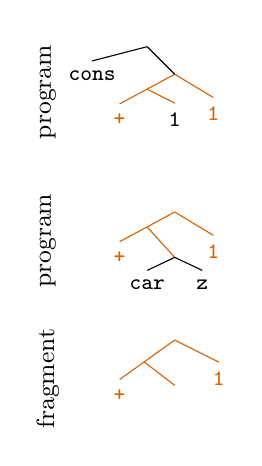
\begin{tikzpicture}[scale=0.7]
    %% \node[rotate=30] at (-2,0) {\begin{tabular}{c}
    %%     \footnotesize Program:\\
    %%     \code{($\lambda$ (x) (+ (- x) 1))}
    %% \end{tabular}};
    %\node at (,0.5) {\code{cons}};
    \node [rotate=90] at (-2.3,-0.5) {\small program};
    
          \node(l1) at (0,0) {};
  \node[color=pop3](p1) at (-1,-1) {\code{+}};
  \node[color=pop3](n1) at (0.7,-0.9) {\code{1}};
  \node(x1) at (0,-1) {\code{1}};
  \draw[color=pop3] (l1.south) -- (p1.north);
  \draw[color=pop3] (l1.south) -- (n1.north);
  \draw[color=pop3] (-0.5,-0.45) -- (x1.north);

  \node(t) at (-0.5,0.5) {};
  \draw (l1.south) -- (t.south);
  \node(c) at (-1.5,-0.2) {\code{cons}};
  \draw (t.south) -- (c.north);
  
%    \draw  (l1.south) -- (-0.5,0.5);

  %% \node(c) at (-0.5,-1.5) {\code{-}};
  %% \node(z) at (0.5,-1.5) {\code{x}};

  %% \draw (0,-1) -- (c.north);
  %% \draw (0,-1) -- (z.north);
  
  \begin{scope}[shift={(0,-2.5)}]
      \node(l1) at (0,0) {};
  \node[color=pop3](p1) at (-1,-1) {\code{+}};
  \node[color=pop3](n1) at (0.7,-0.9) {\code{1}};
  %\node(x1) at (0,-1) {};
  \draw[color=pop3] (l1.south) -- (p1.north);
  \draw[color=pop3] (l1.south) -- (n1.north);
  \draw[color=pop3] (-0.5,-0.45) -- (0,-1);


  \node(c) at (-0.5,-1.5) {\code{car}};
  \node(z) at (0.5,-1.5) {\code{z}};

  \draw (0,-1) -- (c.north);
  \draw (0,-1) -- (z.north);

  \node [rotate=90] at (-2.3,-0.7) {\small program};
  
  \end{scope}

\begin{scope}[shift={(0,-5)}]
  \node[pop3](p1) at (-1,-1) {\code{+}};
  \node[pop3](n1) at (0.8,-0.7) {\code{1}};
  \node[pop3](a) at (0,-1) {\code{ }};
  %\node(x1) at (0,-1) {};
  \draw[pop3] (0,0) -- (p1.north);
  \draw[pop3] (0,0) -- (n1.north);
  \draw[pop3] (-0.55,-0.4) -- (a.north);
  \node [rotate=90] at (-2.3,-0.7) {\small fragment};

  \end{scope}

\end{tikzpicture}
  \end{minipage}
\hspace{0.1cm}\begin{tabular}{ll}
    \toprule
    Example programs in frontiers&Proposed $\lambda$-expression\\\midrule
    \begin{tabular}{l}
      \code{($\lambda$ ($\ell$) (map ($\lambda$ (x) (index x $\ell$))}\\
      \phantom{\code{($\lambda$ ($\ell$) (map }}\code{(range (- (length $\ell$) 1))))}\\
      \code{($\lambda$ ($\ell$) (map ($\lambda$ (x) (index x $\ell$))}\\
      \phantom{\code{($\lambda$ ($\ell$) (map }}\code{(range (+ 1 1))))}\\
    \end{tabular}&
    \begin{tabular}{l}
      \code{(map ($\lambda$ (x) (index x $\ell$))}\\
      \phantom{\code{(map)}}\code{(range $\alpha$))}\\
    \end{tabular}\\\midrule
    \begin{tabular}{l}
      \code{($\lambda$ (s) (map ($\lambda$ (x)}\\
      \hspace{0.4cm}\code{ (if (= x '.') '-' x))) s)}\\
      \code{($\lambda$ (s) (map ($\lambda$ (x) }\\
      \hspace{0.4cm}\code{ (if (= x '-') ',' x))) s)}\\
      \end{tabular}&
    \begin{tabular}{l}      \code{($\lambda$ (s) (map ($\lambda$ (x)}\\\hspace{0.2cm}\code{   (if (= x $\alpha$) $\beta$ x))) s)}
      \end{tabular}
\\\bottomrule\\
\end{tabular}
\caption{\textbf{Left:} syntax trees of two programs sharing common structure,
highlighted in {\orange{orange}},
  from which we extract a fragment and add it to the DSL (bottom). \textbf{Right:} actual programs,
  from which we extract fragments that  (top) slice from the beginning of a list or (bottom) perform character substitutions.}\label{fragmentExample}
\end{figure}
\begin{figure}%{R}{0.6\textwidth}\vspace{-1cm}
\centering  \begin{minipage}{0.9\textwidth}    
    \begin{algorithm}[H]
      \caption{The \system Algorithm}
      \label{mainAlgorithm}
      \begin{algorithmic}
        \STATE {\bfseries Input:} Initial DSL $\mathcal{D}$, set of tasks $X$, iterations $I$
        \STATE \textbf{Hyperparameters:} Enumeration timeout $T$
        %     \STATE \textbf{Output:} DSL $\mathcal{D}$, weight vector $\theta$, recognition model $q(\cdot)$
        \STATE Initialize $\theta\gets \text{uniform}$ %, $q_0(\cdot ) = \theta_0$
        \FOR{$i=1$ {\bfseries to} $I$}
        %     \FOR{$x:\tau\in X$}
        \STATE For each task $x\in X$, set  $\mathcal{F}^{\theta}_x\gets \{p| p\in
        \text{enum}(\mathcal{D},\theta,T)\text{ if }\probability[x|p] > 0\}$
        \footnotesize{\hfill(\textbf{Explore})}
        \STATE $q\gets \text{train recognition model, maximizing }\mathcal{L}_{\text{RM}}$ (see Sec.~\ref{recognitionSection})\hfill(\footnotesize{\textbf{Compile}})
        \STATE For each task $x\in X$, set $\mathcal{F}^{q}_x\gets\{p|p\in
        \text{enum}(\mathcal{D},q(x),T)\text{ if }\probability[x|p] > 0\}$
        \footnotesize{\hfill\textbf{(Explore)}}
        
        \STATE $\mathcal{D},\theta\gets $induceDSL$(\{\mathcal{F}^{\theta}_x\cup\mathcal{F}^{q}_x\}_{x\in X})$  (see Sec.~\ref{grammarInductionSection})\footnotesize{\hfill\textbf{(Compress)}}
        %% \STATE Define $Q_x(z) \propto \begin{cases}
        %%   \probability[x|z]\probability[z|\mathcal{D}_i,\theta_i]&x\in \mathcal{F}_x\\
        %%   0&x\not \in \mathcal{F}_x
        %% \end{cases}
        \ENDFOR
        \STATE \textbf{return} $\mathcal{D},\theta,q$
      \end{algorithmic}
    \end{algorithm}
  \end{minipage}
\end{figure}
To define the prior distribution over $(\mathcal{D},\theta})$, we penalize the syntactic complexity of the $\lambda$-calculus expressions in the DSL, defining $    \probability[\mathcal{D}]\propto\exp(-\lambda\sum_{p\in \mathcal{D}}\text{size}(p) )$ where $\text{size}(p)$  measures the size of the syntax tree of program $p$,
and place a symmetric Dirichlet prior over the weight vector $\theta$.
%% , $  \probability[\theta|\mathcal{D}] = \text{Dir}(\theta|\alpha)$, where
 %% $\alpha$ is a concentration parameter controlling the smoothness of the prior over $\theta$.
%Alg.~\ref{grammarInductionAlgorithm} specifies the DSL induction algorithm.

%% Although this  may seem 
%% very similar to estimating the parameters of a probabilistic context free grammar,
%% for which we have effective approaches like the Inside/Outside algorithm~\cite{international2000derivation},
%% our DSLs are context-sensitive due to the presence of variables
%% in the programs and also due to the polymorphic typing system.
%% In the Supplement we derive a tractable MAP estimator for $\theta$.
Putting all these ingredients together, Alg.~\ref{mainAlgorithm} describes how we combine program search,
recognition model training, and DSL induction.
For added robustness,
we interleave an extra program search step (Exploration) before training the recognition model,
and just enumerate from the prior $(\mathcal{D},\theta)$ during this extra Exploration step.
 
\begin{comment}
\subsection{Implementing \system}

Alg.~\ref{mainAlgorithm} describes how we combine program search,
recognition model training, and DSL induction.
We note the following implementation details:
(1) We perform an search cycle before each compression and compilation  cycle.
(2) On the first iteration, we do \emph{not} train the recognition model on samples from
the generative model because a generative model has not yet been learned --
we instead train the network to only maximize $\mathcal{L}_{\text{AE}}$.
%% (3) Because the frontiers can grow very large,
%% we only keep around the top $10^4$ programs $p$ in each frontier $\mathcal{F}_x$
%% with the highest likelihood $\probability[x,p|\mathcal{D},\theta]$.
(3) During both DSL induction and neural net training, we calculate Eq.~\ref{AIC} and $\mathcal{L}_{\text{RM}}$
by only summing over the top $K$
programs in $\mathcal{F}_x$ as measured by $\probability[x,p|\mathcal{D},\theta]$ -- we found that $K = 2$ sufficed.
(4) For added robustness, we enumerate programs from both the generative model $(\mathcal{D},\theta)$ and the recognition model.
\end{comment}



%\section{Experiments}
%% We first present our experimental results qualitatively,
%% illustrating the learned DSLs.
%% We then show quantitative results (Sec.~\ref{quantitative})
%% comparing \system with lesioned versions
%% of our model that are analogous to prior work.

\pagebreak
\section{Programs that manipulate sequences}\label{sequences}
We apply \system to list processing (Section~\ref{listSection}) and text editing (Section~\ref{textSection}).
For both these domains we use a bidirectional GRU~\cite{cho2014learning} for
the recognition model, and initially provide the system with a generic set
of list processing primitives:
\code{foldr}, \code{unfold}, \code{if}, \code{map}, \code{length},
\code{index}, \code{=}, \code{+}, \code{-}, \code{0}, \code{1}, \code{cons},
\code{car}, \code{cdr}, \code{nil}, and \code{is-nil}.

\vspace{0.5cm}

\subsection{List Processing}\label{listSection}
Synthesizing programs that manipulate data structures is a widely studied
problem in the programming languages community~\cite{feser2015synthesizing}.
%with applications to computer aided programming~\cite{solar2008program}.
We consider this problem within the context of learning functions that
manipulate lists, and which also perform arithmetic operations upon lists of numbers.


\begin{wrapfigure}{r}{0.55\textwidth}\centering
  \begin{tabular}{lll}
    \toprule
    Name & Input & Output \\\midrule
    repeat-2 & [7\, 0] & [7\, 0\, 7\, 0] \\
    drop-3 & [0\, 3\, 8\, 6\, 4] & [6\, 4] \\
    rotate-2 & [8\, 14\, 1\, 9] & [1\, 9\, 8\, 14] \\
    count-head-in-tail & [1\, 2\, 1\, 1\, 3] & 2 \\
    keep-mod-5 & [5\, 9\, 14\, 6\, 3\, 0] & [5\, 0] \\
    product & [7\, 1\, 6\, 2] & 84 \\
    \bottomrule
  \end{tabular}
  \captionof{table}{Some tasks in our list function domain. See the
  supplement for the complete data set.}\label{listexamples}
\end{wrapfigure}
We created 236 human-interpretable list manipulation tasks, each with 15
input/output examples (Tbl.~\ref{listexamples}).
Our data set is interesting in three major ways: many of the tasks require
complex solutions; the tasks were not generated from some latent DSL; and
the agent must learn to solve these complicated problems from only 236
tasks.
Our data set assumes arithmetic operations as well as sequence operations,
so we additionally provide our system with the following arithmetic
primitives: \code{mod}, \code{*}, \code{>}, \code{is-square},
\code{is-prime}.

We evaluated \system on  random 50/50 test/train split.
Interestingly, we found that the recognition model provided little benefit for the training
tasks. However, it yielded faster search times on held out tasks, allowing
more tasks to be solved before timing out.
The system composed 38 new subroutines, yielding a more expressive DSL more closely matching the
domain (left of Tbl.~\ref{initialExampleDSL}, right of
Fig.~\ref{fragmentExample}). See the supplement for a complete list of
DSL primitives discovered by \systemEnding.

\subsection{Text Editing}\label{textSection}
Synthesizing programs that edit text is a classic problem in the
programming languages and AI literatures~\cite{menon2013machine,lau2001programming},
and algorithms that learn text editing programs ship in Microsoft Excel~\cite{gulwani2011automating}.
This prior work presumes a hand-engineered DSL.
We show \system can instead start out with generic sequence manipulation
primitives and recover many of the higher-level building blocks that have
made these other text editing systems successful.

Because our enumerative search procedure cannot generate string
constants, we instead enumerate programs with string-valued
parameters.  For example, to learn a program that prepends ``Dr.'', we
enumerate $\text{\code{(}}f_3\code{ string s)}$ -- where $f_3$ is the
learned appending primitive (Fig.~\ref{initialExampleDSL}) --- and then
define $\probability[x|p]$ by approximately marginalizing out the
string parameters via a simple dynamic program.
In Sec.~\ref{regressionSection}, we will use a similar trick to
synthesize programs containing real numbers, but using gradient
descent instead of dynamic programming.

We trained our system on a corpus of 109 automatically generated text editing tasks, with 4 input/output examples each.
After three iterations, it assembles a DSL containing a dozen new functions (center of Fig.~\ref{initialExampleDSL}) that let it solve 
all of the training tasks.
But, how well does the  learned DSL generalized to real text-editing scenarios?
We tested, but did not train, on the 108 text editing problems from the SyGuS~\cite{alur2016sygus} program synthesis competition. Before any learning,
\system solves 3.7\% of the problems with an average search time of 235 seconds.
After learning,
it solves 74.1\%, and does so much faster,
solving them in an average of 29 seconds.
As of the 2017 SyGuS competition,
the best-performing algorithm solves 79.6\% of the problems.
But, SyGuS comes with a
different hand-engineered DSL \emph{for each text editing problem}.\footnote{SyGuS text editing problems also prespecify the set of allowed string constants for each task. For these experiments, our system did not use this assistance.}
Here  we learned a single DSL
that applied generically to
all of the tasks,
and perform comparably to the best
prior work.

\section{Symbolic Regression: Programs from visual input}\label{regressionSection}
We apply \system
to symbolic regression problems.  Here, the
agent observes points along the curve of a function, and must write a
program that fits those points.  We initially equip our learner with
addition, multiplication, and division, and task it with solving
100 symbolic regression problems, each either a polynomial of degree
1--4 or a rational function.  The recognition model is a
convolutional network that observes an image of the target function's
graph (Fig.~\ref{functions}) --- visually, different kinds of
polynomials and rational functions produce different kinds of graphs,
and so the recognition model can learn to look at a graph and predict
what kind of function best explains it.  A key difficulty, however, is
that these problems are best solved with programs containing real
numbers.  Our solution to this difficulty is to enumerate
 programs with real-valued parameters, and then fit those
parameters by automatically differentiating through the programs the
system writes and use gradient descent to fit the parameters.
We define the likelihood model, $\probability[x|p]$, by assuming a Gaussian noise model for the input/output examples,
and penalize the use of real-valued parameters using the BIC~\cite{Bishop:2006:PRM:1162264}.

\begin{wrapfigure}{r}{0.45\textwidth}\vspace{-0.5cm} \newcommand{\functionSize}{1.5cm}\centering
  
\includegraphics[width = \functionSize]{figures/functions/6.png}
  
\includegraphics[width = \functionSize]{figures/functions/48.png}
  
\includegraphics[width = \functionSize]{figures/functions/102.png}
  
\includegraphics[width = \functionSize]{figures/functions/116.png}\\
  \vspace{1pt}
\includegraphics[width = \functionSize]{figures/functions/181.png}
  
\includegraphics[width = \functionSize]{figures/functions/160.png}
  
\includegraphics[width = \functionSize]{figures/functions/149.png}
    
\includegraphics[width = \functionSize]{figures/functions/187.png}
  \caption{Recognition model input for symbolic regression. DSL learns subroutines for polynomials (top row) and rational functions (bottom row) while the recognition  model jointly learns to look at a graph of the function (above) and predict which of those subroutines best explains the observation.}\label{functions}\vspace{-2cm}
\end{wrapfigure}
\system learns a DSL containing 13 new functions,
most of which are templates for polynomials of different orders or ratios of polynomials.
It also learns to find programs that minimize the number of continuous degrees of freedom.
For example, it learns to represent linear functions with the program
\code{(* real (+ x real))}, which has two continuous degrees of freedom, and represents quartic functions using the invented DSL primitive $f_4$ in the rightmost column of Fig.~\ref{initialExampleDSL}
which has five continuous parameters.
This phenomenon arises from our Bayesian framing --- both the implicit bias towards shorter programs and the likelihood model's BIC penalty.


\section{Quantitative Results}\label{quantitative}

We compare with ablations of our model on held out tasks.
The purpose of this ablation study is 
both to examine the role of each component of \systemEnding,
as well as to compare with
prior approaches in the literature:
a head-to-head
comparison of program synthesizers is complicated by the fact that
each system, including ours, makes idiosyncratic 
assumptions about the space of programs and the statement of tasks.
Nevertheless, much prior work can be modeled within our setup. 
We compare with the following ablations (Tbl~\ref{baselineComparisons};
Fig~\ref{learningCurves}):
\\\noindent \textbf{No NN:} lesions the recognition model.
\\\noindent \textbf{NPS}, which does not learn the DSL,
instead learning the recognition model
from samples drawn from the fixed DSL.
We call this NPS (Neural Program Synthesis)
because this is closest to how
RobustFill~\cite{devlin2017robustfill} and DeepCoder~\cite{balog2016deepcoder} are trained.
\\\noindent \textbf{SE}, which lesions the recognition model and restricts the DSL  learning algorithm to
only add \textbf{S}ub\textbf{E}xpressions of programs in the frontiers to the DSL. This is how most prior approaches have learned libraries of functions~\cite{Dechter:2013:BLV:2540128.2540316,DBLP:conf/icml/LiangJK10,DBLP:conf/ecai/LinDETM14}.
\\\noindent \textbf{PCFG}, which lesions the recognition model and does not learn the DSL,
but instead learns the parameters of the DSL ($\theta$), learning the parameters of a PCFG while not learning any of the structure.
\\\noindent \textbf{Enum}, which enumerates a frontier without any learning --- equivalently, our first exploration step.

\begin{wraptable}{r}{0.55\textwidth}
\vspace{-10pt}
%% This radically shrinks the table
\tabcolsep=2.5pt
\renewcommand{\arraystretch}{0.5}
\begin{tabular}{lcccccc}
  \toprule& Ours& 
    No NN & SE&NPS & PCFG & Enum \\
  \midrule
  \multicolumn{7}{c}{\emph{List Processing}}\\
  \midrule
  \% solved&\textbf{94\%} & 
  79\% &71\%&35\%&62\%&37\%\\
  Solve time&  88s&39s&11s&35s&44s&20s\\
  \midrule
  \multicolumn{7}{c}{\emph{Text Editing}}\\
  \midrule
  \% solved&\textbf{74\%} &43\% &30\%&33\%&0\%&4\%\\
  Solve time& 29s&49s % FIXME: 65 in the table but 49 on the graph? 65s
  &38s&80s&--&235s\\
  \midrule
  \multicolumn{7}{c}{\emph{Symbolic Regression}}\\
  \midrule
  \% solved&   \textbf{84\% }&75\%&62\%&38\%&38\%&37\% \\
  Solve time&  24s& 40s  &28s&31s&55s&29s\\
  \bottomrule
  \end{tabular}
\caption{\% held-out test tasks solved. Solve time: averaged over solved
  tasks.  %SE: NPS: trained like RobustFill/DeepCoder.  PCFG: model w/o
  %structure learning.  Enum: model w/o any learning.  %% MDL:
  %% $-\expect\left[\probability[x|p] \right]$. For domains other than
  %% symbolic regression MDL is 0 nats.
  %% For symbolic regression MDL is a
  %% proxy for \# of continuous parameters.
}\vspace{-1cm}\label{baselineComparisons} \end{wraptable}
%For each domain,
We are interested both in how many tasks the
agent can solve and how quickly it can find those solutions.
Tbl.~\ref{baselineComparisons}
compares our model against these alternatives.
We consistently
improve on the baselines,
and also find that lesioning the recognition model
impairs the convergence of the algorithm,
causing it to hit a lower `plateau' after which it stops solving new tasks, following an initial spurt of learning (Fig.~\ref{learningCurves}) -- without the neural network, search becomes intractable.
This lowered `plateau' supports a view of the recognition model as a way of amortizing the cost of search.


\begin{figure}\centering
  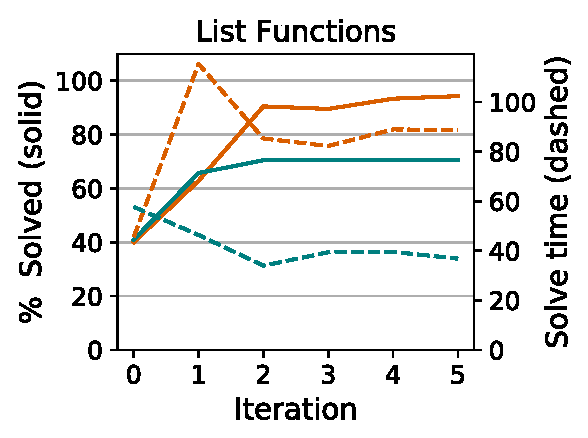
\includegraphics[width = 4.35cm]{figures/listLearningCurve_color.eps}
  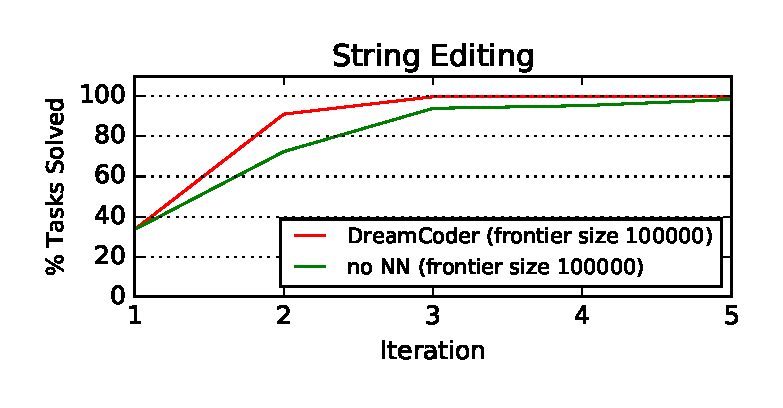
\includegraphics[width = 4.5cm]{figures/textLearningCurve.eps}
  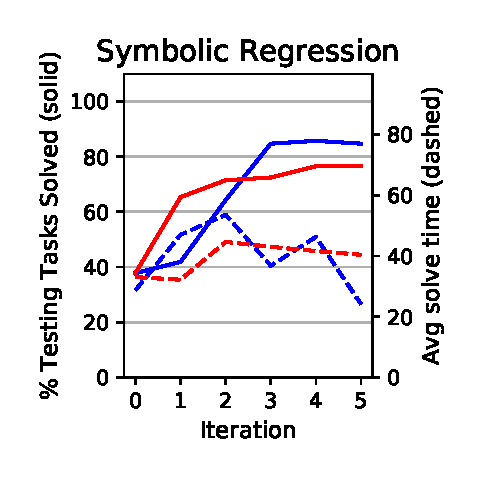
\includegraphics[width = 4.5cm]{figures/rationalCurve.eps}
  \caption{Learning curves for \system both with (\orange{in orange}) and without
  (\teal{in teal}) the recognition model. Solid lines: \% holdout testing tasks solved. Dashed lines: Average solve time.}\label{learningCurves}
\end{figure}

\section{Related Work}
 Our work is far from the first for learning to learn programs,
 an idea that goes back to Solomonoff~\cite{solomonoff1989system}:

 \noindent \textbf{Deep learning:} Much recent work in the ML community has
 focused on creating neural networks that regress from
 input/output examples to programs~\cite{devlin2017robustfill,devlin2017neural,menon2013machine,balog2016deepcoder}. %This family of work is closest to our RF/DC baseline.
\systemEnding's recognition model draws heavily from this line of work, particularly from~\cite{menon2013machine}.
We see these prior works as operating in a different regime: typically, they train with strong supervision (i.e., with annotated ground-truth programs) on massive data sets (i.e., hundreds of millions~\cite{devlin2017robustfill}).
 Our work   considers a weakly-supervised regime where ground truth programs are not provided and
 the agent must learn from at most a few hundred tasks,
 which is facilitated by our ``Helmholtz machine'' style recognition model.%(Sec.~\ref{recognitionSection}).
 
 \noindent \textbf{Inventing new subroutines for program induction:}
 Several program induction algorithms, most prominently the EC algorithm~\cite{Dechter:2013:BLV:2540128.2540316}, take as their goal to learn new, reusable subroutines that are shared in a multitask setting. We find this work inspiring and motivating,
 and extend it along two dimensions: (1) we propose a new algorithm for
 inducing reusable subroutines, based on Fragment Grammars~\cite{tim};
 and (2) we show how to combine these techniques with bottom-up neural recognition models.
 Other instances of this related idea are~\cite{DBLP:conf/icml/LiangJK10}, Schmidhuber's OOPS model~\cite{schmidhuber2004optimal}, MagicHaskeller~\cite{katayama2015towards}, Bayesian program merging~\cite{hwang2011inducing}, and predicate invention in Inductive Logic Programming~\cite{DBLP:conf/ecai/LinDETM14}.
 Concurrent with this work, closely related ideas were applied to mining `code idioms' from imperative programs~\cite{8355713}
 and for synthesizing functional programs from natural language~\cite{Alex}.
 
 
\noindent\textbf{Bayesian Program
 Learning:} Our work is an instance of
 Bayesian Program
 Learning (BPL; see~\citep{lake2015human,Dechter:2013:BLV:2540128.2540316,ellis2016sampling,DBLP:conf/icml/LiangJK10,ellis2015unsupervised}). Previous BPL systems have largely assumed a fixed DSL (but see~\cite{DBLP:conf/icml/LiangJK10}),
 and our contribution here is a general way of doing BPL with less hand-engineering of the DSL.
 
 \section{Limitations of EC$^2$}

 We have presented an algorithm that, starting from relatively little,
 learned to solve program synthesis problems in three
 different domains.  However, our system was also given (and also,
 critically \emph{needs}) a corpus of training tasks to solve for each
 domain.  Is constructing (or curating) corpra of tasks any easier or
 better than hand-engineering DSLs?  In the immediate future, we
 expect some degree of hand-engineering of DSLs to continue, especially
 in domains where humans have strong intuitions about the underlying
 system of domain specific concepts, like text editing. However, if
 program induction is to become a standard part of the AI toolkit,
 then, in the long-term, we need to build agents that autonomously
 acquire the domain specific knowledge needed to navigate a new
 domain.  So, through the lens of program synthesis, EC$^2$ carries
 the limitation that it requires a high-quality corpus of training
 tasks; but, for the program-induction approach to AI, this limitation
 is natural.

 The particular implementation of EC$^2$ developed here
 inherits a key limitation from a specific arbitrary engineering decision:
 our enumerative program search strategy cannot possibly
 scale to large bodies of code, even with a good recognition model --- but one could in principle replace
 our enumerative approach with stochastic search~\cite{schkufza2013stochastic,DBLP:books/daglib/0070933},
 constraint solving~\cite{solar2008program}, type-directed synthesis~\cite{polikarpova2016program},
 or other techniques from the program synthesis community.
 
 
 
 

 \section{Discussion}

%\parbox{0.58\textwidth}{

%\paragraph{Outlook.}
We contribute an algorithm, \systemEnding, that learns to program by
bootstrapping a DSL with new domain-specific primitives that the algorithm
itself discovers, together with a neural recognition model that learns how to
efficiently deploy the DSL on new tasks. We believe this integration of top-down
symbolic representations and bottom-up neural networks --- both of them learned
--- helps make program induction systems more generally useful for AI. Many
directions remain open.
%\paragraph{Future.}
Two immediate goals are to integrate more sophisticated neural recognition
models~\cite{devlin2017robustfill} and program
synthesizers~\cite{solar2008program}, which may improve performance in some
domains over the generic methods used here.
%% We are in the process of applying our algorithm to generative programs and
%% prototyped this with a turtle-like domain: Figure~\ref{geomCompiled} gives some
%% preliminary results for turtle graphics  --- see Section 1 of the supplementary material for more
%% details.
Another direction is to explore DSL meta-learning: can we find a
\emph{single} universal primitive set that could effectively bootstrap DSLs for
new domains, including the three domains considered,  but also many others?
%% }\hfill
%% \begin{minipage}{0.4\textwidth}
%%   \centering
%%   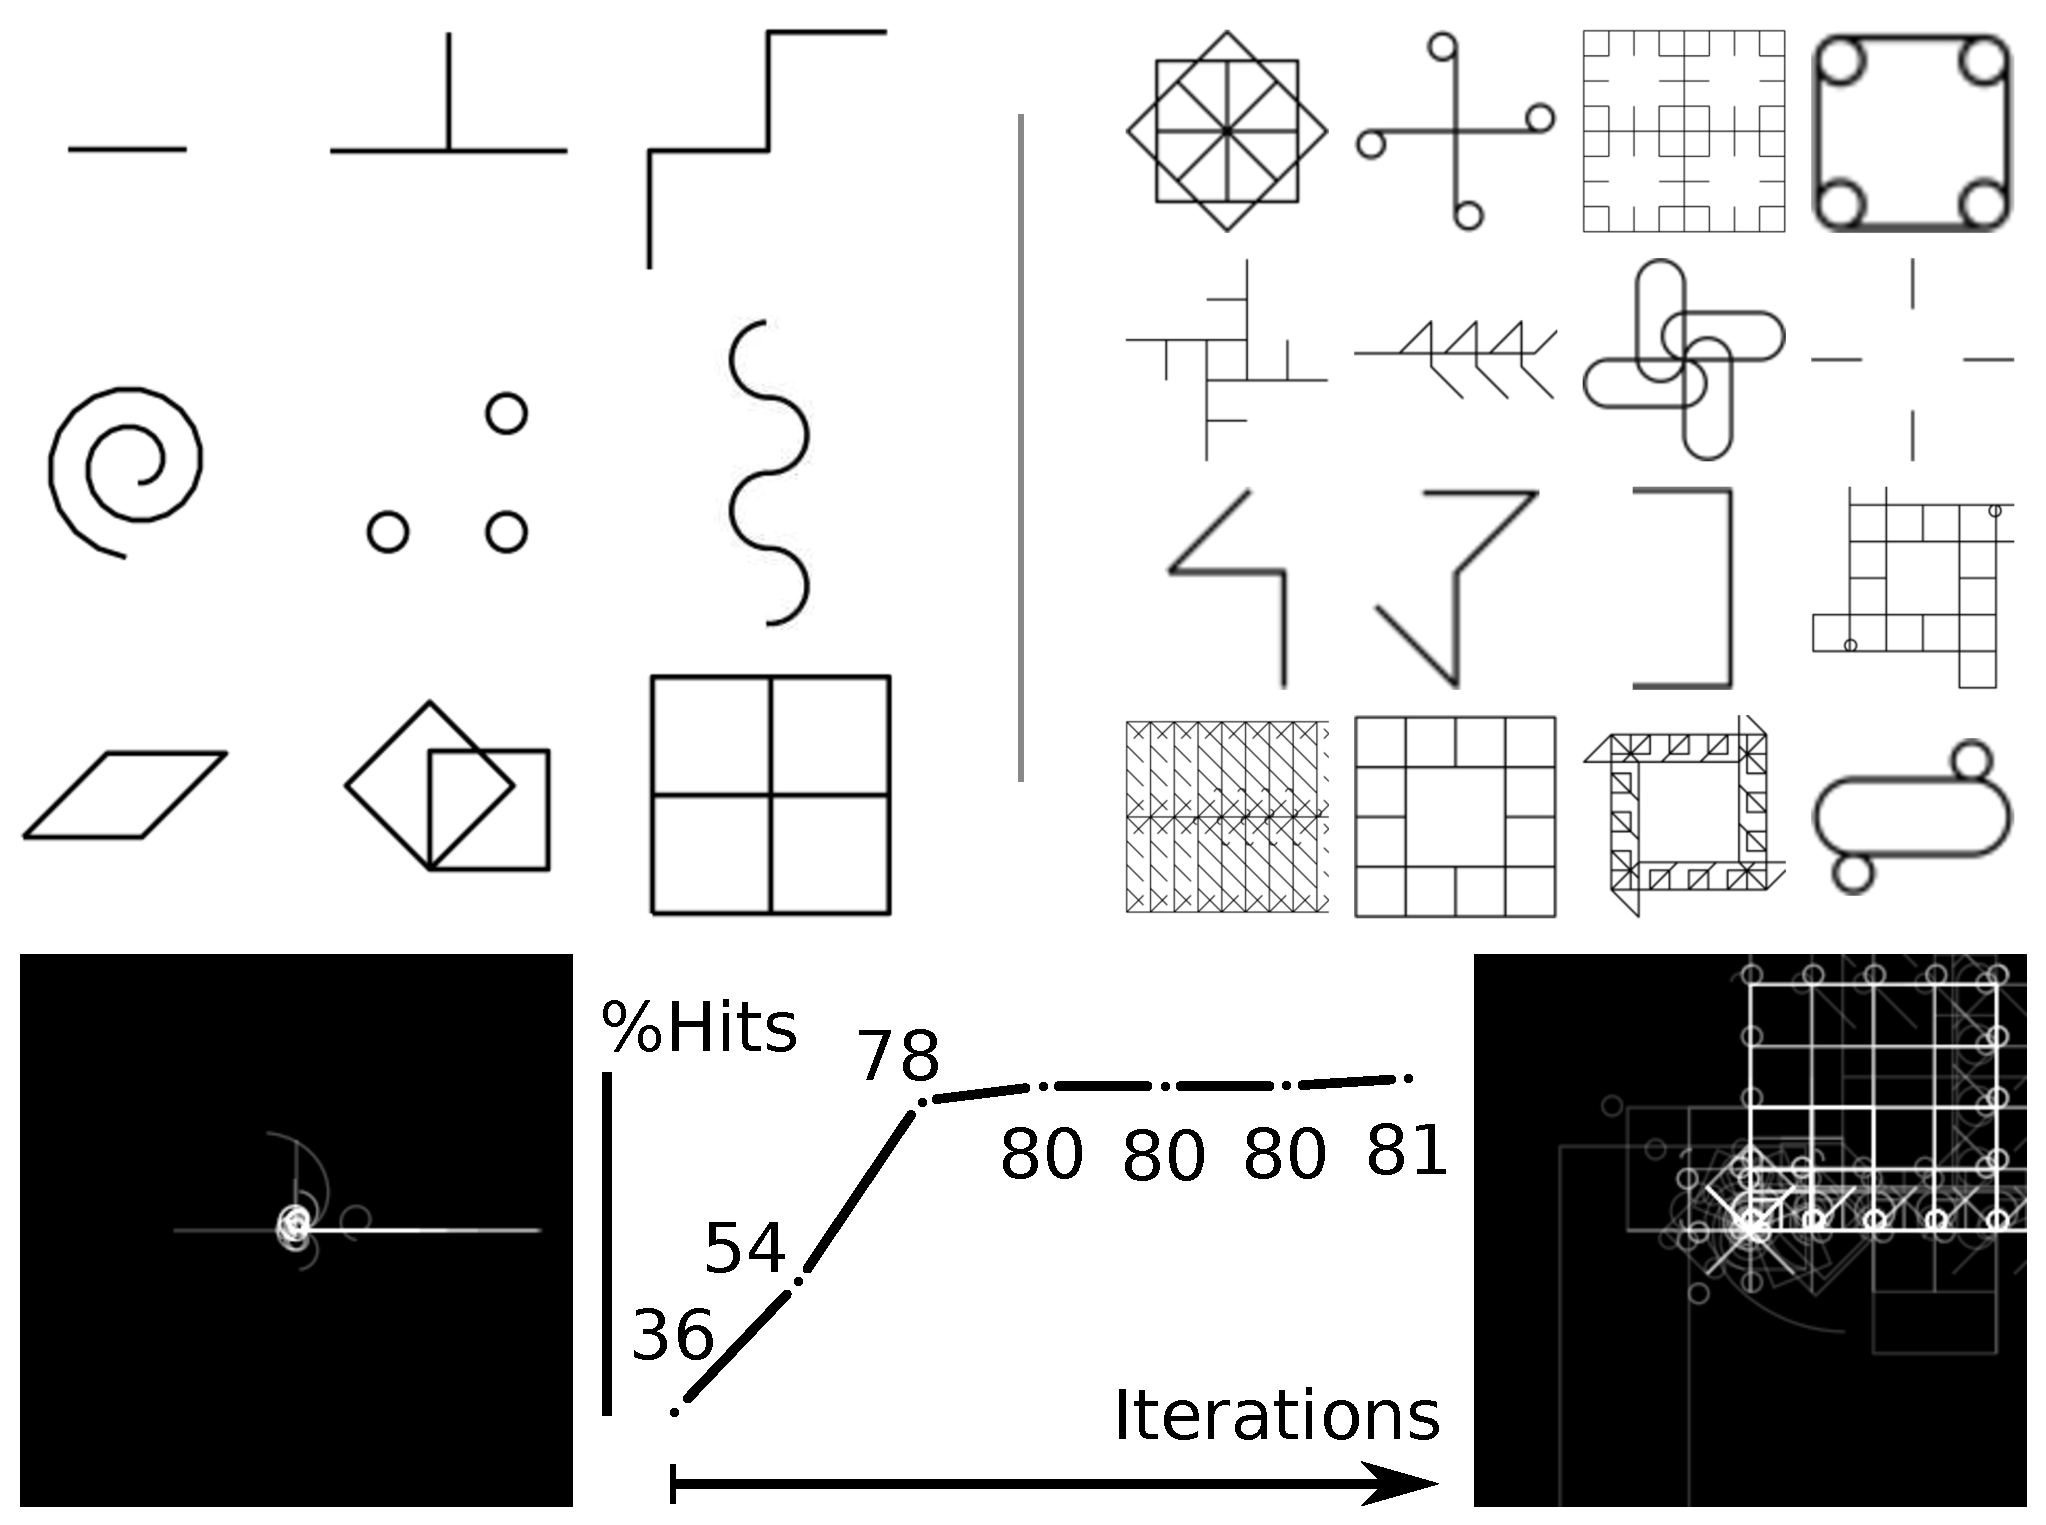
\includegraphics[width=\textwidth]{figures/geomCompiled.eps} 
%%   \captionof{figure}{
%%   Top left: Example training tasks. Top right: samples from the learned DSL.
%%  Bottom: \% holdout testing tasks solved (middle), on sides are the averaged samples from the DSL
%%   before any training (left) and after last iteration (right).}
%% \label{geomCompiled}
%% \end{minipage}

\subsubsection*{Acknowledgments} We are grateful for collaborations with Eyal Dechter, whose EC algorithm directly inspired this work, and for funding from the NSF GRFP, the MUSE program (Darpa grant FA8750-14-2-0242),
and an AWS ML Research Award.


\bibliographystyle{unsrt}
{\small \bibliography{main}}
\end{document}
